% @author: Felix Hekhorn
\documentclass[
  english,		% Sprache
  a4paper,		% Papierformat
  11pt,			% Schriftgröße (default 10pt)
  %DIV=12,		% Seiteneinteilung
  DIV=12,
  titlepage,
  toc=bibnumbered,
  parskip=full,  	% Absätze (full,half,false -+*)
  headings=normal,
  BCOR=12mm,
  numbers=noenddot
]{scrartcl}
%\documentclass[a4paper,10pt]{article}
\usepackage{scrtime,scrlfile,scrpage2}

\usepackage[status=draft,inline,nomargin,marginclue]{fixme}
%\usepackage[status=final]{fixme}

\usepackage[utf8]{inputenc}
%\usepackage[ngerman]{babel} % Sprache 
\usepackage[ngerman,english,main=english]{babel} % Sprache 
\selectlanguage{english}
\usepackage{amsmath, amssymb}

%\usepackage{graphicx} % Grafiken einbinden
% The following is needed in order to make the code compatible
% with both latex/dvips and pdflatex.
\ifx\pdftexversion\undefined
\usepackage[dvips]{graphicx}
\else
\usepackage[pdftex]{graphicx}
\DeclareGraphicsRule{*}{mps}{*}{}
\fi

%\usepackage[left=2cm,right=2cm,top=2.5cm,bottom=3cm]{geometry}
\usepackage{color}
\usepackage{bbm}

\usepackage{pdflscape}
\usepackage{ulem}
\usepackage{url}
\usepackage{caption}
\usepackage{subcaption}
\usepackage{array}
\usepackage{multirow}
\usepackage{listings}
\usepackage{placeins}
\usepackage{csquotes}

\usepackage{siunitx} % SI Einheiten
\usepackage[version=3]{mhchem}
%\sisetup{
%	exponent-product = \!\cdot\!,
%	output-product = \cdot,
%	list-final-separator =  { und } ,
%	list-pair-separator = { und } ,
%	range-phrase = { bis },
%	output-decimal-marker = {,},
%	separate-uncertainty = true,
%	group-digits = false
%}

%\usepackage{simplewick}
%\usepackage{feynmf}
\usepackage{slashed}
\usepackage{hepnames}

%\usepackage{biblatex}
\usepackage[numbers]{natbib}
%\bibliographystyle{natdin}
%\bibliographystyle{kp}
\bibliographystyle{utphys}

\usepackage{hyperref}
%\hypersetup{colorlinks=false}
\usepackage{tabularx}

\providecommand{\abs}[1]{\left|#1\right|}
\providecommand{\VektorV}[3]{
\!\left(\!\!
\begin{array}{c}
#1 \\ #2 \\ #3
\end{array}\!\!
\right)\!
}

\providecommand{\Det}[9]{
	\begin{vmatrix}
	    #1 & #2 & #3 \\
	    #4 & #5 & #6 \\
	    #7 & #8 & #9 \\	    
	\end{vmatrix}
}

\DeclareMathOperator{\Grad}{\text{grad}}
\DeclareMathOperator{\Div}{\text{div}}
\DeclareMathOperator{\Rot}{\text{rot}}
\DeclareMathOperator{\tr}{\text{tr}}

\DeclareMathOperator{\acos}{\text{arccos}}
\DeclareMathOperator{\asin}{\text{arcsin}}
\DeclareMathOperator{\atanh}{\text{artanh}}
\DeclareMathOperator{\x}{\times}
\DeclareMathOperator{\cdt}{\!\cdot\!}
\DeclareMathOperator{\del}{\partial}
\DeclareMathOperator{\EqualClaim}{\stackrel{!}{=}}
\DeclareMathOperator{\equivals}{\mathrel{\widehat{=}}}
\providecommand{\Nabla}[0]{\vec\nabla}
\providecommand{\ex}[1]{e^{#1}}
\providecommand{\EE}[1]{\cdot 10^{#1}}
\providecommand{\FT}[1]{\mathcal{FT}\left[#1\right]}
\providecommand{\Mel}[1]{\mathcal{M}\left[#1\right]}
\providecommand{\invMel}[1]{\mathcal{M}^{-1}\left[#1\right]}

\providecommand{\dt}[0]{\Derive t}
\providecommand{\dx}[0]{\Derive x}
\providecommand{\Derive}[1]{\DeriveN{#1}{}}
\providecommand{\DeriveN}[2]{\DeriveNF {#1}{#2}{}}
\providecommand{\DeriveF}[2]{\DeriveNF {#1}{}{#2}}
\providecommand{\DeriveNF}[3]{\frac {d^{#2}#3} {d #1^{#2}}}
\providecommand{\dtP}[0]{\DeriveP t}
\providecommand{\dxP}[0]{\DeriveP x}
\providecommand{\DeriveP}[1]{\DerivePN{#1}{}}
\providecommand{\DerivePF}[2]{\DerivePNF {#1} {} {#2}}
\providecommand{\DerivePN}[2]{\DerivePNF {#1} {#2} {} }
\providecommand{\DerivePNF}[3]{\frac {\partial^{#2}#3} {\partial #1^{#2}}}
\providecommand{\DerivePMF}[3]{\frac {\partial^{2}#3} {\partial #1 \partial #2}}
\providecommand{\e}[1]{\hat{e}_{#1}}
\providecommand{\pFq}[2]{{}_{#1}F_{#2}}

\providecommand{\bra}[1]{\langle#1\rvert}
\providecommand{\ket}[1]{\lvert#1\rangle}
\providecommand{\bracket}[2]{\langle#1\vert#2\rangle}
\providecommand{\normOrd}[1]{\,:\!#1\!:\,}
\providecommand{\wContr}[3]{\contraction{}{#1}{#2}{#3}#1#2#3}

\DeclareMathOperator{\und}{\text{UND}}
\DeclareMathOperator{\oder}{\text{ODER}}

\DeclareMathOperator{\Md}{\mathcal M}
\DeclareMathOperator{\Ld}{\mathcal L}
\DeclareMathOperator{\Hd}{\mathcal H}
\DeclareMathOperator{\Nd}{\hat {\mathcal N}}
\DeclareMathOperator{\To}{\hat {\mathcal T}}

\DeclareMathOperator{\ijI}{\mathit{ij},\mathbf{I}}
\DeclareMathOperator{\MSbar}{\overline{\text{MS}}}


\DeclareRobustCommand{\PQ}{\HepGenParticle{Q}{}{}\xspace} % quark
\DeclareRobustCommand{\PaQ}{\HepGenAntiParticle{Q}{}{}\xspace} % anti-quark


\begin{document}

\section{Introduction}
\section{Introduction}

\begin{frame}{Introduction - Heavy Quarks (HQ)}
\begin{itemize}
\item Heavy Quarks (HQ): $\Pcharm (m_{\Pcharm}=\SI{1.5}{\GeV})$, $\Pbottom (m_{\Pbottom}=\SI{4.75}{\GeV})$, $\Ptop (m_{\Ptop}=\SI{175}{\GeV})$
\item EIC will reach region with HQ relevant to structure functions
\item compare unpolarized case @HERA: at small $x$ $\sim 30\%$ charm contributions
\item<2-> measure $\Delta g$ as dominated by PGF
\item<2-> first NLO computation of polarized process
\end{itemize}
\begin{itemize}
\item<3-> need improved charm tagging
\item<3-> full inclusive cross section is complicated to reconstruct
\item<3-> no hadronization here
\end{itemize}
\end{frame}

\begin{frame}{Introduction - Heavy Quarks (HQ)}
\newcolumntype{w}{>{\centering\arraybackslash} m{.7\linewidth} }
\newcolumntype{i}{>{\centering\arraybackslash} m{.3\linewidth} }
\begin{tabular}{wi}
\begin{itemize}
%\setlength{\itemindent}{-1em}
\item scale of hard process is in a pertubative regime $m>\Lambda_{QCD}$
\item finite mass $m$ ensures full inclusive cross sections
\item<2-> full $m^2$ dependence makes computations complicated: phase space + matrix elements
\item<2-> 2-scale problem: $\ln\left(\frac{s-4m^2}{4m^2}\right)$ and/or $\ln(Q^2/m^2)$
\item<2-> keep analytic expressions
\end{itemize}
&
\only<beamer>{\includegraphics[width=.27\textwidth]{img/c2}}
\end{tabular}
\end{frame}

\begin{frame}{Introduction - DIS Setup}
\[\Pem(l_1)+h(p) \to \Pem(l_2) + \PaQ(p_2) + X[\PQ]\]
\newcolumntype{w}{>{\centering\arraybackslash} m{.74\linewidth} }
\newcolumntype{i}{>{\centering\arraybackslash} m{.26\linewidth} }
\hspace{-.5cm}\begin{tabular}{iw}
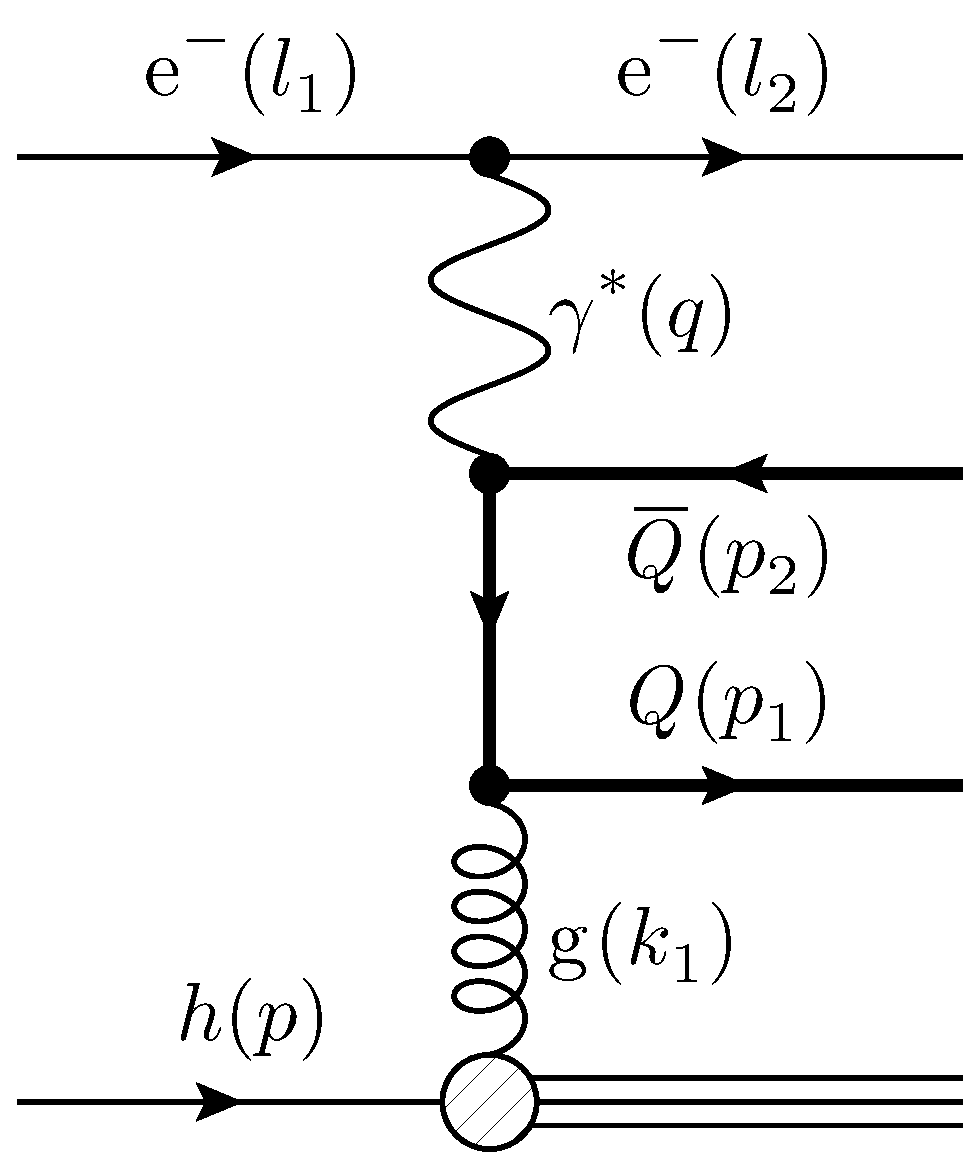
\includegraphics[width=.25\textwidth]{img/DIS.eps} &
\begin{itemize}
\item $S_h = (p+l_1)^2 = x\,y\,Q^2,\,x,\,y,$\\
$Q^2 = -q^2 = - (l_1-l_2)^2 \ll M_Z^2$
\item unpolarized cross section:\\
$\frac{d^2\sigma}{dx dy} = \frac{2\pi \alpha^2}{x y Q^2}\left(Y_+F_2(x,Q^2) - y^2F_L(x,Q^2)\right)$\\
$2xF_1(x,Q^2) = F_2(x,Q^2) - F_L(x,Q^2)$
\item polarized cross section:\\
$\frac{d^2\Delta\sigma}{dx dy} = \frac{4\pi \alpha^2}{x y Q^2}Y_-\cdot 2xg_1(x,Q^2)$
\item with $Y_\pm = 1 \pm (1-y)^2$
\item $[k=T]\to 2xF_1$, $[k=L]\to F_L$ and $[k=P]\to 2xg_1$
\end{itemize}
\end{tabular}
\end{frame}

%%%
\iffalse
\begin{frame}{Introduction - Experimental Setups}
\begin{center}
\newcolumntype{C}{>{\centering\arraybackslash} m{3.6cm} } 
\begin{tabular}{C|C|C}
\Pelectron-\APelectron-annihilation (SIA) & deep inelastic scattering (DIS) & Drell-Yan process (DY)\\
%SIA & DIS & DY\\
\hline
\vspace{3pt}
$\Pelectron+\APelectron \to \PaQ + X[\PQ]$ &
\vspace{3pt}
$\Pl+h \to \Pl' + \PaQ + X[\PQ]$ &
\vspace{3pt}
$h + h' \to \PaQ + X[\PQ]$ \\
\hline
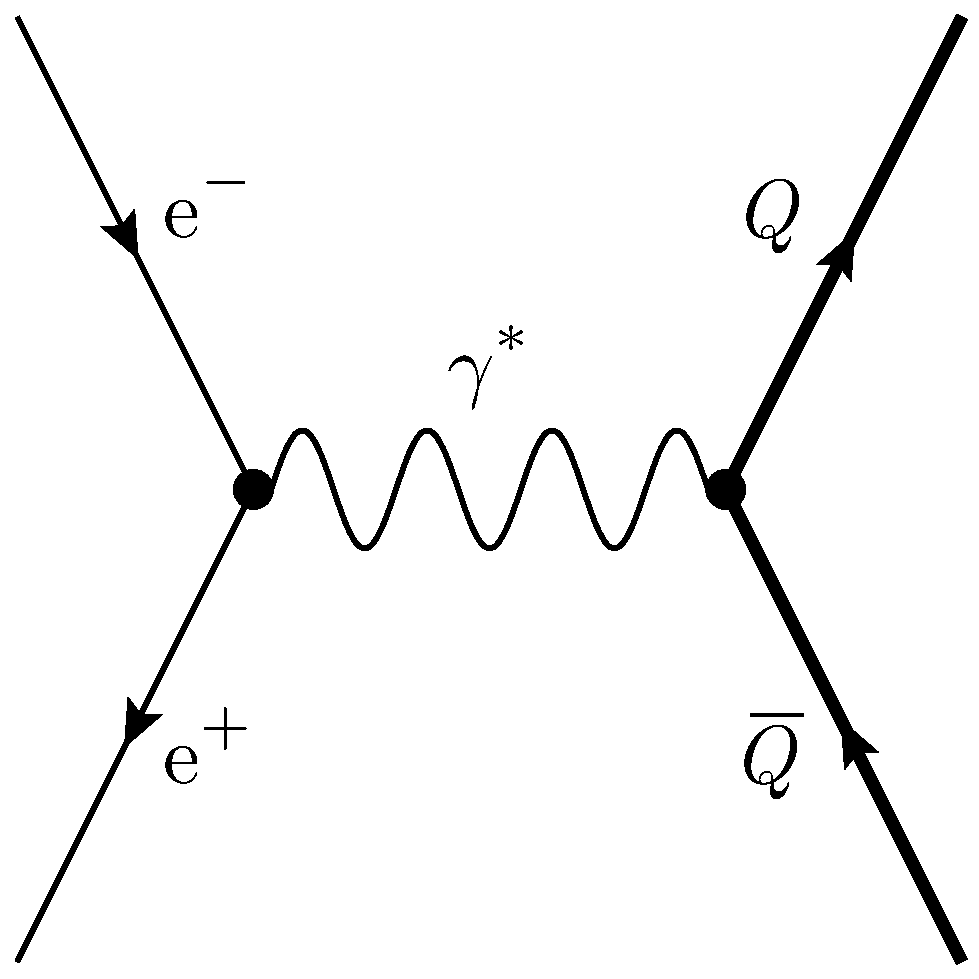
\includegraphics[width=.25\textwidth]{img/SIA.eps} & 
\vspace{.2cm}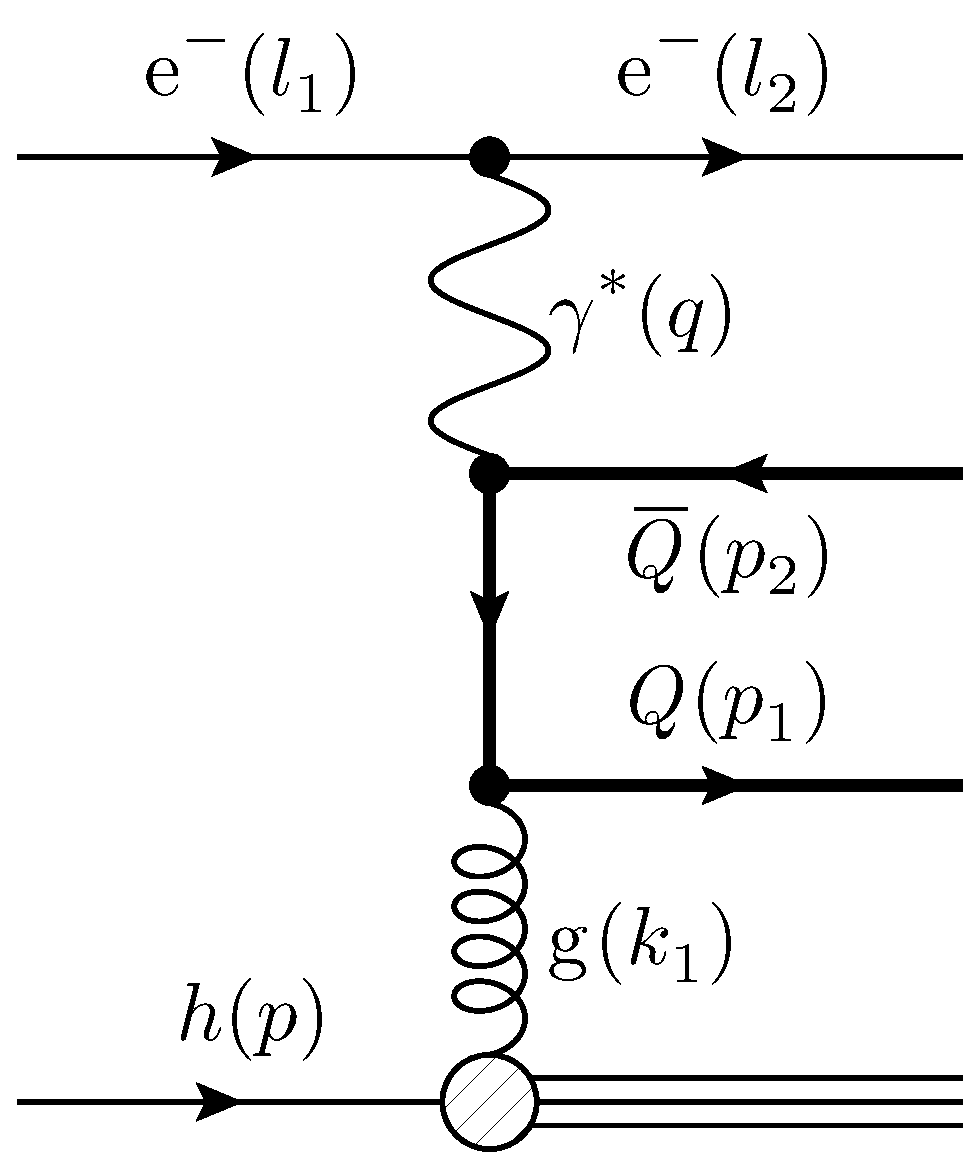
\includegraphics[width=.25\textwidth]{img/DIS.eps} & 
\vspace{.2cm}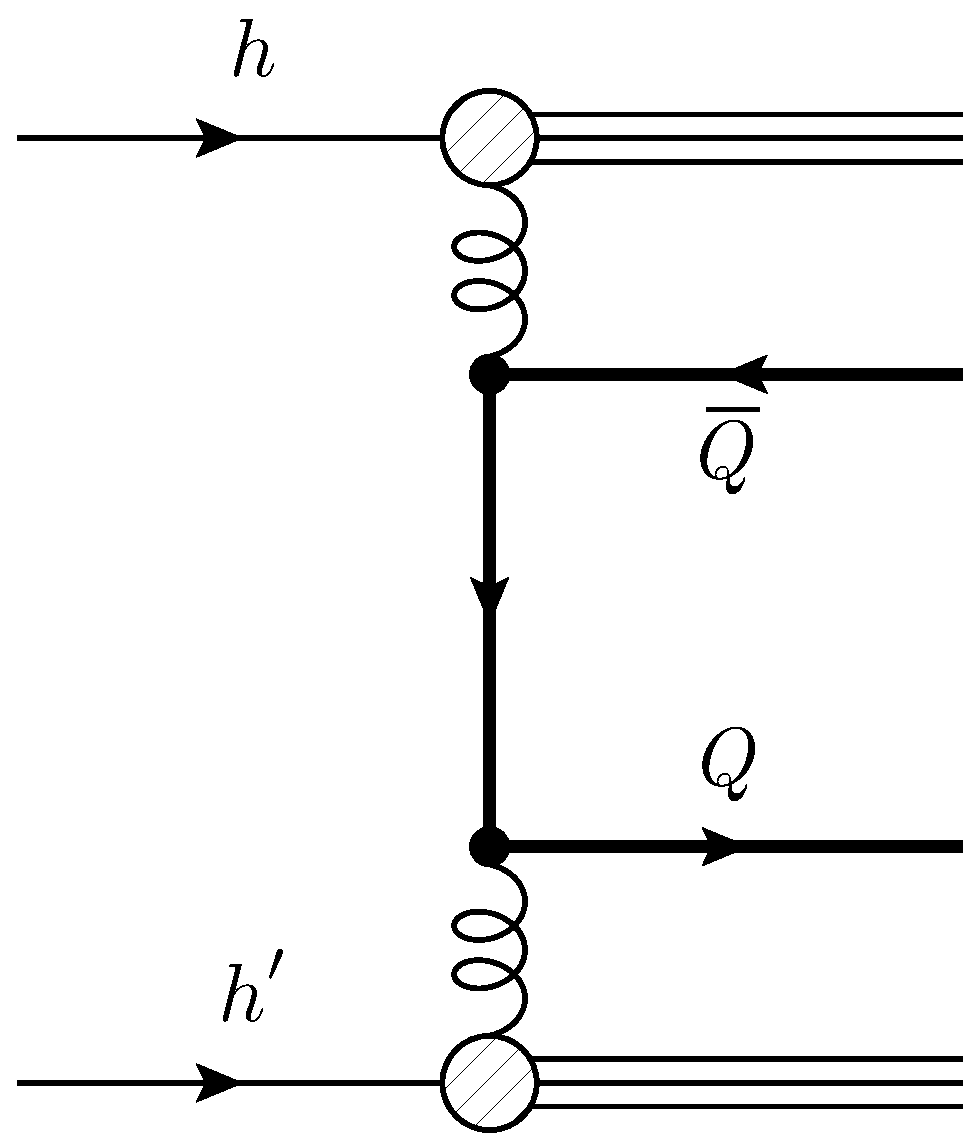
\includegraphics[width=.25\textwidth]{img/DY.eps} \\
\hline
LEP, ILC & \vspace{2pt} HERA, COMPASS, EIC & Tevatron, LHC\\
\hline
gluon & factorization & top, Higgs
\end{tabular}
\end{center}
\end{frame}

\begin{frame}{Introduction - Structure Functions}
\begin{align}
&\text{cross section (xs):}&\frac{d^2\sigma}{dx dy} &= \frac{2\pi y \alpha^2}{Q^4} L^{\mu\nu} W_{\mu\nu}\\
&\text{hadronic tensor:}&W_{\mu\nu} &= \left(-g_{\mu\nu} + \frac{q_\mu q_\nu}{q^2}\right) F_1(x,Q^2) + \frac{P_\mu P_\nu}{P\cdot q} F_2(x,Q^2) \nonumber\\
&& & \hspace{20pt} + i \epsilon_{\mu\nu\alpha\beta} \frac{q^{\alpha}S^{\beta}}{P\cdot q} g_1(x,Q^2)\\
&&F_L(x,Q^2) &= F_2(x,Q^2) - 2xF_1(x,Q^2)\\
&\text{unpolarized xs:}&\frac{d^2\sigma}{dx dy} &= \frac{2\pi \alpha^2}{x y Q^2}\left(Y_+F_2(x,Q^2) - y^2F_L(x,Q^2)\right)\\
&\text{polarized xs:}&\frac{d^2\Delta\sigma}{dx dy} &= \frac{4\pi \alpha^2}{x y Q^2}Y_-\cdot 2xg_1(x,Q^2)\\
&&Y_\pm &= 1 \pm (1-y)^2
\end{align}
\end{frame}
\fi
%%%


\section{Leading Order Calculations}
In leading order we have to consider photon-gluon-fusion (PGF), that is
\begin{equation}
\Pggx(q;\sigma_q) + \Pg(k_1;\sigma_{k_1}) \rightarrow \PQ(p_1)+\PaQ(p_2)
\end{equation}
with two contributing diagrams depicted in figure \fxerror{todo}. The result can then be written as
\begin{equation}
\hat\sum_{k,\sigma}\mathcal P_{k}^{\mu\mu'}\sum_{j=1}^2\Md^{(0)}_{j,\mu}(\sigma_{k_1},\sigma_q)\Md^{(0)*}_{j,\mu'}(\sigma_{k_1},\sigma_q) = 8g^2\mu_D^{-\epsilon}e^2e_H^2 N_C C_F B_{k,QED}
\end{equation}
where $g$ and $e$ are the strong and electromagnetic coupling constants respectively, $\mu_D$ is an arbitray mass parameter introduced to keep the couplings dimensionless and $e_H$ is the magnitude of the heavy quark in units $e$. Further $N_C$ corresponds to the gauge group $SU(N_C)$ and the color factor $C_F=(N_C^2-1)/(2N_C)$ refers to the second Casimir constant of the fundamental representation for the quarks. We then find:
\begin{align}
B_{G,QED} &= \frac{t_1}{u_1} + \frac{u_1}{t_1} + \frac{4m^2s'}{t_1u_1}\left(1-\frac{m^2s'}{t_1u_1}\right)
+\frac{2s'q^2}{t_1u_1} +\frac{2q^4}{t_1u_1} + \frac{2m^2q^2}{t_1u_1}\left(2-\frac{{s'}^2}{t_1u_1}\right)\nonumber\\
 &\hspace{20pt}+\epsilon\left\{ -1 + \frac{{s'}^2}{t_1u_1} + \frac{s'q^2}{t_1u_1} -
\frac{q^4}{t_1u_1} - \frac{m^2q^2{s'}^2}{t_1^2u_1^2} \right\} + \epsilon^2\frac{{s'}^2}{4t_1u_1}\\
B_{L,QED} &= -\frac{4q^2}{s'}\left(\frac s {s'} - \frac{m^2s'}{t_1u_1}\right)\\
B_{P,QED} &= \frac 1 2\left(\frac{t_1}{u_1}+\frac{u_1}{t_1}\right)\left(\frac{2m^2 s'}{t_1u_1}-1 - \frac{2q^2}{s'}\right)\\
B_{k,QED} &= B^{(0)}_{k,QED} + \epsilon B^{(1)}_{k,QED} + \epsilon^2 B^{(2)}_{k,QED}
\end{align}

By using eq. (\ref{eq:PartonicStructureTensor0}) we can derive the $n$-dimensional $2\rightarrow 2$ phase space
\begin{equation}
dPS_2 = \!\int\!\!\frac{d^{n}p_1}{(2\pi)^{n-1}}\frac{d^{n}p_2}{(2\pi)^{n-1}}\Theta(p_{1,0})\delta(p_1^2-m^2)\Theta(p_{2,0})\delta(p_2^2-m^2)(2\pi)^n\delta^{(n)}(k_1+q-p_1-p_2)
\end{equation}
that can be solved by using the center-of-mass system (CMS) of the incoming particles\cite{Bojak:2000eu}
\begin{align}
q &= \left(\frac {s+q^2}{2\sqrt s},0,0,-\frac{s-q^2}{2\sqrt s},\hat 0\right) &
k_1 &= \frac {s-q^2}{2\sqrt s}\left(1,0,0,1,\hat 0\right)
\end{align}
such that $q+k_1=(\sqrt s,\vec 0)$ and $k_1^2 = 0$. For the outgoing particles it follows
\begin{align}
p_1 &= \frac{\sqrt s} 2 \left(1,0,\beta\sin\theta,\beta\cos\theta,\hat 0\right)&
p_2 &= \frac{\sqrt s} 2 \left(1,0,-\beta\sin\theta,-\beta\cos\theta,\hat 0\right)
\end{align}
such that $p_1+p_2 = (\sqrt s,\vec 0)$ and $p_1^2 = p_2^2=m^2$. Finally we have to use the $n$-sphere
\begin{equation}
d^nx = \frac{2\pi^{n/2}}{\Gamma(n/2)}x^{n-1} dx= \frac{\pi^{n/2}}{\Gamma(n/2)}(x^2)^{(n-2)/2} dx^2
\end{equation}
and arrive at the well known result\cite{Laenen1993162}
\begin{align}
dPS_2 &= \frac {\delta(s'+t_1+u_1)} {2s'\Gamma((n-2)/2)(4\pi)^{(n-2)/2}}\left(\frac{(t_1u_1'-s'm^2)s' - q^2t_1^2}{s'^2}\right)^{(n-4)/2}\,dt_1du_1\\
 &= \delta(s'+t_1+u_1) h_2(n)\,dt_1 du_1\\
h_2(4+\epsilon) &= \frac {2\pi S_\epsilon} {s'\Gamma(1+\epsilon/2)}\left(\frac{(t_1u_1'-s'm^2)s' - q^2t_1^2}{s'^2}\right)^{\epsilon/2}
\end{align}
with $S_\epsilon = (4\pi)^{(-2-\epsilon/2)}$.

The final double differential LO partonic cross section can then be written as
\begin{align}
{s'}^2\frac{d^2\sigma_{k,\Pg}^{(0)}(s',t_1,u_1,q^2)}{dt_1du_1} &= 2^6\alpha\alpha_s e_H^2 K_{\Pg\Pgg}N_CC_F E_k(\epsilon) b_k(\epsilon)\delta(s'+t_1+u_1) \frac{\pi^3S_\epsilon}{\Gamma(1+\epsilon/2)}  \nonumber\\
 &\hspace{20pt} \left(\frac{(t_1u_1'-s'm^2)s' - q^2t_1^2}{m^2{s'}^2}\right)^{\epsilon/2}\left(\frac{\mu_D^2}{m^2}\right)^{-\epsilon/2} B_{k,QED}
\end{align}
where we used $e^2=4\pi\alpha$ and $g^2=4\pi\alpha_s$ and introduced the arbitrary mass parameter $\mu_D$ to keep the strong coupling dimensionless. The color average is given by $K_{\Pg\Pgg} = 1/(N_C^2-1)$.

From the results above we can easily obtain the \textit{total} LO partonic cross sections
\begin{align}
\sigma_G^{(0)}(s,q^2,m^2) &=-4\pi\alpha\alpha_s e_H^2 K_{\Pg\Pgg}N_CC_F\frac 1 {{s'}^3}\left((s^2+q^4+4m^2 s)\beta + (s^2+q^4-4m^2(2m^2-s'))\ln(\chi)\right)\\
\sigma_L^{(0)}(s,q^2,m^2) &=16\pi\alpha\alpha_s e_H^2 K_{\Pg\Pgg}N_CC_F\left(\frac{-q^2s}{{s'}^3}\right)\left(\beta + \frac{2m^2}{s}\ln(\chi)\right)\\
\sigma_P^{(0)}(s,q^2,m^2) &=4\pi\alpha\alpha_s e_H^2 K_{\Pg\Pgg}N_CC_F\frac 1 {{s'}^2}\left((3s+q^2)\beta + (s+q^2)\ln(\chi)\right)
\end{align}
from which we also see
\begin{equation}
\lim_{s\rightarrow 4m^2} \sigma_T^{(0)}(s',q^2) = 4\pi\alpha\alpha_s e_H^2 K_{\Pg\Pgg}N_CC_F\frac{\beta}{4m^2-q^2} + O(\beta^3) = \lim_{s\rightarrow 4m^2} \sigma_P^{(0)}(s',q^2)
\end{equation}
\fxerror{shift to partonic?}


\section{Next-To-Leading Order Calculations}
\subsection{One Loop Virtual Contributions}
\begin{align}
M_{\vec \kappa}^{(1),V}&=\hat {\mathcal P}_{\vec \kappa}^{\Pgg,\mu\mu'}\hat {\mathcal P}_{\kappa_2}^{\Pg,\nu\nu'}\sum_{j,j'}2\text{Re}\left[\Md^{(1),V}_{j,\mu\nu}\left(\Md^{(0)}_{j',\mu'\nu'}\right)^*\right] \nonumber\\
 &= 8g^4\mu_D^{-\epsilon}e^2e_H^2 N_C C_FC_\epsilon\left( C_A V_{\vec \kappa,\tOK} + 2C_F V_{\vec \kappa,\tQED}\right)
\end{align}
where $C_\epsilon = \exp(\epsilon/2(\gamma_E-\ln(4\pi)))/(16\pi^2)$ and $C_A$ is the second Casimir constant of the adjoint representation for the gluon (that introduces a non-abelian part).

The full expressions for the $V_{\vec \kappa,\tOK},V_{\vec \kappa,\tQED}$ are quite complicated and are too long to be presented here, nevertheless the arising poles are quite compact:
\begin{align}
V_{\vec \kappa,\tOK} &= -2B_{\vec \kappa,\tQED}\left(\frac 4 {\epsilon^2} + \left(\ln(-t_1/m^2) + \ln(-u_1/m^2) +\frac{s-2m^2}{s\beta}\ln(\chi)\right)\frac 2 \epsilon \right) + O(\epsilon^0)\\
V_{\vec \kappa,\tQED} &= -2B_{\vec \kappa,\tQED}\left(1-\frac{s-2m^2}{s\beta}\ln(\chi)\right)\frac 2 \epsilon + O(\epsilon^0)
\end{align}
The above results already include the mass renormalization that we have performed \textit{on-shell}, so all ultra-violet poles have been removed. For the renormalization of the strong coupling we use the $\MSbar_m$ scheme defined in \cite{Bojak:2000eu} and so the full (remaining) renormalization can be achieved by
\begin{align}
\frac{d^2\sigma_{\vec \kappa,\Pg}^{(1),V}}{dt_1du_1} &=\left.\frac{d^2\sigma_{\vec \kappa,\Pg}^{(1),V}}{dt_1du_1} \right|_{\text{bare}}+ 4\pi\alpha_s(\mu_R^2)C_\epsilon\left(\frac{\mu_D^2}{m^2}\right)^{-\epsilon/2}\left[\left(\frac 2 \epsilon +\ln(\mu_R^2/m^2)\right)\beta_0^f +\frac 2 3 \ln(\mu_R^2/m^2)\right]\frac{d^2\sigma_{\vec \kappa,\Pg}^{(0)}}{dt_1du_1}
\end{align}
with $\mu_R$ the renormalization scale introduced by the RGE, $\beta_0^f = (11C_A- 2n_{f})/3$ the first coefficient of the beta function and $n_f$ the number of \textit{total} flavours (i.e. $n_{lf}=n_f-1$ active (light) flavours and one heavy flavour). The double poles occuring in $V_{\vec \kappa,\tOK}$ are introduced by the diagrams \fxerror{do} when the soft and collinear singularities coincide.

The partonic cross section is given by
\begin{align}
d\sigma_{\vec \kappa,\Pg}^{(1),V} &= \frac 1 {2s'}\frac 1 2 E_{\kappa_2}(\epsilon) M_{\vec \kappa}^{(1),V} \dPSTwo
\end{align}


\subsection{Single Gluon Radiation}
\label{sec:NLO.g}
In addition to the virtual corrections we have to consider the radiation of an additional gluon at next-to-leading order, i. e., the $2\to 3$ process
\begin{equation}
b(q) + \Pg(k_1) \rightarrow \PQ(p_1)+\PaQ(p_2) + \Pg(k_2),\quad b\in\{\Pggx,\PZx\}
\end{equation}
All contributing diagrams are depicted in figure \fxerror{do} and the result can be written as
\begin{align}
M_{\vec \kappa}^{(1),\Pg} &= \hat {\mathcal P}_{\vec \kappa}^{b,\mu\mu'}\hat {\mathcal P}_{\kappa_2}^{\Pg,\nu\nu'}\sum_{j,j'}\Md^{(1),\Pg}_{j,\mu\nu}\left(\Md^{(1),\Pg}_{j',\mu'\nu'}\right)^*\\
 &= 8g^4\mu_D^{-2\epsilon}e^2e_H^2 N_C C_F\left( C_A R_{\vec \kappa,\tOK} + 2C_F R_{\vec \kappa,\tQED}\right)
\end{align}

The required $n$-dimensional phase space $\dPSThree$ is given by
\begin{align}
\dPSThree &= \frac{S_\epsilon^2}{\Gamma(1+\epsilon)s'} \frac{s_4^{1+\epsilon}}{(s_4+m^2)^{1+\epsilon/2}}\left(\frac{(t_1u_1'-s'm^2)s' - q^2t_1^2}{s'^2}\right)^{\epsilon/2}\! dt_1 du_1 d\Omega_n
\end{align}
with $d\Omega_n = \sin^{n-3}(\theta_1)d\theta_1\sin^{n-4}(\theta_2)d\theta_2$.

Again when integrating the phase space angles the expressions become quite lengthy, but the collinear poles can be given in a compact form by
\begin{align}
\frac{s_4}{2\pi(s_4+m^2)}\int\!d\Omega_n \,C_A R_{\vec \kappa,OK} &=-\frac 2 {u_1}B_{\vec \kappa,\tQED}\left(\!\begin{array}{l}s'\rightarrow x_1s'\\t_1\rightarrow x_1 t_1\end{array}\!\!\right) P^{(0),H}_{\kappa_2,\Pg\Pg}(x_1)\frac 2 \epsilon + O(\epsilon^0) \label{eq:ROKPoles}
\end{align}
with $x_1 = -u_1/(s'+t_1)$ and the hard part of the LO Altarelli-Parisi splitting functions $P^{(0),H}_{\kappa_2,\Pg\Pg}$\cite{Altarelli:1977zs,Vogelsang:1995vh}:
\begin{align}
P^{(0),H}_{F_2,\Pg\Pg}(x) = P^{(0),H}_{F_L,\Pg\Pg}(x) = P^{(0),H}_{xF_3,\Pg\Pg}(x) &= C_A\left(\frac 2 {1-x} + \frac 2 x - 4 + 2x - 2x^2\right) \label{eq:PFggH}\\
P^{(0),H}_{2xg_1,\Pg\Pg}(x) = P^{(0),H}_{g_4,\Pg\Pg}(x) = P^{(0),H}_{g_L,\Pg\Pg}(x) &= C_A\left(\frac 2 {1-x} - 4x + 2\right) \label{eq:PgggH}
\end{align}
The hard abelian QED part $R_{\vec \kappa,\tQED}$ does not contain collinear poles.

The spin and color averaged partonic cross section for the real corrections to the PGF process is then given by
\begin{align}
d\sigma_{\vec \kappa,\Pg}^{(1),R} &= \frac 1 {2s'}\frac 1 2 E_{\kappa_2}(\epsilon)K_{\Pg\Pgg} M_{\vec \kappa}^{(1),\Pg} \dPSThree
\end{align}

From these expressions we can obtain the soft gluon limit $k_2\rightarrow 0$ and seperate their calculations:
\begin{equation}
\lim_{k_2\rightarrow 0}\left(C_A R_{\vec \kappa,\tOK} + 2C_F R_{\vec \kappa,\tQED}\right) = \left(C_A S_{\vec \kappa,\tOK} + 2C_F S_{\vec \kappa,\tQED}\right) + O(1/s_4,1/s_3,1/t')
\end{equation}
where
\begin{align}
S_{\vec \kappa,\tOK}  &= 2\left(\frac{t_1}{t's_3} + \frac{u_1}{t's_4}-\frac{s-2m^2}{s_3s_4}\right)B_{\vec \kappa,\tQED}\\
S_{\vec \kappa,\tQED} &= 2\left(\frac{s-2m^2}{s_3s_4} - \frac{m^2}{s_3^2} - \frac{m^2}{s_4^2}\right)B_{\vec \kappa,\tQED}
\end{align}
Note that the einkonal factors multiplying the Born functions $B_{\vec \kappa,\tQED}$ neither depend on the photon's virtuality $q^2$ nor on the projection $\vec \kappa$. 


\subsection{Light Quark Processes}
In next-to-leading order a new production mechanism enters that is induced by a light quark, so we have to consider the process
\begin{equation}
\Pggx(q) + \Pq(k_1) \rightarrow \PQ(p_1)+\PaQ(p_2) + \Pq(k_2)
\end{equation}
All contributing diagrams are depicted in figure \fxerror{do} and the result can be written as
\begin{equation}
\hat {\mathcal P}_{k}^{\Pgg,\mu\mu'}\hat {\mathcal P}_{k}^{\Pq}\sum_{j,j'}{\Md^{(1),q}_{j,\mu}\Md^{(1),q}_{j',\mu'}}^* = 8g^4\mu_D^{-2\epsilon}e^2 N_C C_F\left( e_H^2 A_{k,1} +  e_L^2 A_{k,2} +  e_L e_H A_{k,3} \right)
\end{equation}
where $e_L$ denotes the charge of the light quark $q$ in units of $e$.

The results agree in the photo-production limit ($q^2\rightarrow 0$) with \cite{Bojak:1998zm}.



\section{Mass Factorization}
%All collinear poles in the gluonic subprocess can be removed by mass factorization in the following way:
\fxerror{todo}

The light quark process can be regularized in a complete analogous way:
\fxerror{todo}

The final finite cross sections are then
\begin{align}
d\sigma_{k,\Pg}^{(1),c-} &= 16\cdot \frac 1 {2xs'} \frac {K_{\Pgg\Pg}} 2 b_k{0} \cdot \alpha_S^2e^2e_H^2N_C C_F B_{k,QED}(xk_1) dPS_{2}^{(5)} \nonumber\\
 &\hspace{20pt}\cdot \left( (1-x)P_{k,\Pg\Pg}^{H,(0)}(x)\left(\frac{1}{(1-x)_{\tilde\rho}}\left(\ln(s'/\mu_F^2) + \ln(s'/s) + \ln(\omega/2)\right) \right.\right.\nonumber\\
 &\hspace{120pt} \left.\left. + 2\left(\frac{\ln(1-x)}{1-x}\right)_{\tilde\rho} \right) + 2P_{k,\Pg\Pg}^{H,(1)}(x)\right)
\end{align}
\fxerror{todo}


\fxerror{do}

\section{Partonic Results}
%\fxerror{write partonic}

\clearpage
\pagebreak

\fxerror{do}

\section{Hadronic Results}
%The hadronic reaction to study is deep-inelastic lepton-proton scattering:
\begin{equation}
\Pleptonminus(l_1) + \Pp(p) \rightarrow \Pleptonminus(l_2) + \PQ(p_1)(\PaQ(p_2)) + X
\end{equation}
where one either detects the heavy quark $\PQ$ \textit{or} the heavy anti quark $\PaQ$ and $X$ stands for any final hadronic state allowed by quantum-number conservation. We define then the hadronic Bjorken variables
\begin{equation}
q=l_1-l_2 \quad x=\frac{-q^2}{2p\cdot q} \quad z = \frac{p\cdot q}{p\cdot l_1}
\end{equation}

We can then define the measurable deep-inelastic hadron structure functions
\begin{align}
F_k(x,Q^2,m^2) &= \sum_{n=0}^\infty F_{k}^{(n)}(x,Q^2,m^2)\\
F_{k}^{(n)}(x,Q^2,m^2) &= \sum_{j\in\{\Pg,\Pq,\Paq\}}\int\limits_x^{z_{max}} \frac{dz}{z} f_j(x/z,\mu_F^2) \frac{-q^2}{4\pi^2\alpha} \sigma^{(n)}_{k,j}(s,q^2,m^2)
\end{align}
where $k\in\{G,L,P\}$ denotes as usual projection, $z=Q^2/s'$, $z_{max} = Q^2/(4m^2+Q^2)$ and $f_j(x/z,\mu_F^2)$ denotes parton momentum density functions\cite{Martin:2009iq,PhysRevLett.113.012001}.
We can then split the contributions whether there is a gluon in the initial state $F_{k,g}$ or a (anti)quark $F_{k,q}$. In leading order we find:
\begin{align}
F_{k,g}^{(0)}(x,Q^2,m^2) &= \frac{\alpha_sQ^2}{4\pi^2m^2}e_H^2\int\limits_x^{z_{max}}\frac{dz}{z} f_g(x/z,\mu_F^2) c^{(0)}_{k,g}(\eta,\xi)
\end{align}
In next-to-leading order we find for the gluonic part:
\begin{align}
&F_{k,g}^{(1)}(x,Q^2,m^2) \nonumber\\
 &= \frac{\alpha_s^2Q^2}{\pi m^2}e_H^2\int\limits_x^{z_{max}}\frac{dz}{z} f_g(x/z,\mu_F^2) \left(c_{k,g}^{(1)}(\eta,\xi) + \ln(\mu_F^2/m^2)\bar c_{k,g}^{F,(1)}(\eta,\xi) + \ln(\mu_R^2/m^2)\bar c_{k,g}^{R,(1)}(\eta,\xi)\right)
\end{align}
In next-to-leading order we find for the quark part:
\begin{align}
&F_{k,q}^{(1)}(x,Q^2,m^2) \nonumber\\
 &= \frac{\alpha_s^2Q^2}{\pi m^2}e_H^2\int\limits_x^{z_{max}}\frac{dz}{z} \left(\sum_{j=1}^{n_{lf}}f_{q(j)}(x/z,\mu_F^2)+f_{q(-j)}(x/z,\mu_F^2)\right) \nonumber\\
 &\hspace{120pt} \cdot\left(c_{k,q}^{(1)}(\eta,\xi) + \ln(\mu_F^2/m^2)\bar c_{k,q}^{F,(1)}(\eta,\xi)\right) \nonumber\\
 &\hspace{20pt} + \frac{\alpha_s^2Q^2}{\pi m^2}\int\limits_x^{z_{max}}\frac{dz}{z} \left(\sum_{j=1}^{n_{lf}}e_{q(j)}^2\left(f_{q(j)}(x/z,\mu_F^2)+f_{q(-j)}(x/z,\mu_F^2)\right)\right) d_{k,q}(\eta,\xi)
\end{align}
where we used the PDG particle labeling\cite{Hagiwara:2002fs}: $q(1)=u,q(-1)=\bar u,q(2)=d,q(-2)=\bar d$, \ldots and $e_u = e_c = e_t = 2/3, e_d=e_s=e_b=-1/3$. 

We can then also define some more practical functions:
\begin{align}
F_{2}(x,Q^2,m^2) &= F_{T}(x,Q^2,m^2) + F_{L}(x,Q^2,m^2)\\
 &= F_{G}(x,Q^2,m^2) + \frac 3 2 F_{L}(x,Q^2,m^2)\\
F_1(x,Q^2,m^2) &= (F_{2}(x,Q^2,m^2)-F_L(x,Q^2,m^2))/(2x)\\
 &= \left(F_{G}(x,Q^2,m^2)+\frac 1 2 F_{L}(x,Q^2,m^2)\right)/(2x)\\
g_1(x,Q^2,m^2) &= F_{P}(x,Q^2,m^2)/(2x)
\end{align}
and we define the spin asymmetry
\begin{align}
A_1(x,Q^2,m^2) &= \frac{g_1(x,Q^2,m^2)}{F_1(x,Q^2,m^2)} = \frac{F_P(x,Q^2,m^2)}{F_2(x,Q^2,m^2)-F_L(x,Q^2,m^2)}
\end{align}

For the plots we focused on charm production ($n_{lf}=3$) with $m_c=\SI{1.5}{\GeV}$ and we used the running coupling of \fxerror{cite,do}: We set $\mu_F^2=\mu_R^2=4m^2-q^2$ in analogy to \cite{Laenen1993162}.We used the PDF set MSTW2008nlo90cl\cite{Martin:2009iq,Martin:2009bu,Martin:2010db} provided by LHAPDF\cite{LHAPDF6} for the unpolarized structure functions ($F_2,F_G,F_L$) and DSSV2014\cite{PhysRevLett.113.012001} for the polarized structure function ($F_G$).

\fxerror{shift to appendix?}

\pagebreak
\begin{figure}[ht!]
\centering
\begin{subfigure}[t]{\textwidth}
	\input{img/F0012}
\end{subfigure}\\%
\begin{subfigure}[t]{\textwidth}
	\input{img/F001L}
\end{subfigure}\\%
\begin{subfigure}[t]{\textwidth}
	\input{img/F001P}
\end{subfigure}
\caption{hadronic structure functions $F_{k}(x,Q^2,m_c^2)$ plotted as function of $x$ for different values of $Q^2$ in units of $\si{\GeV^2}$}\label{fig:F001}
\end{figure}

\clearpage
\pagebreak

\fxerror{do}

\section{Summary}
%\input{Summary}
\fxerror{do}

\newpage
\appendix

\bibliography{ref.bib}
\listoffixmes

\end{document}
